\subsection{System-functionalities}




\subsubsection{Data flow diagram}
til opdatering af diagram
- øverste dataflow skal hedde phone nr og kode
- realtime skal ændres til real-time
- gps skal ændres all around til GPS
\begin{figure} [H]
    \centering
    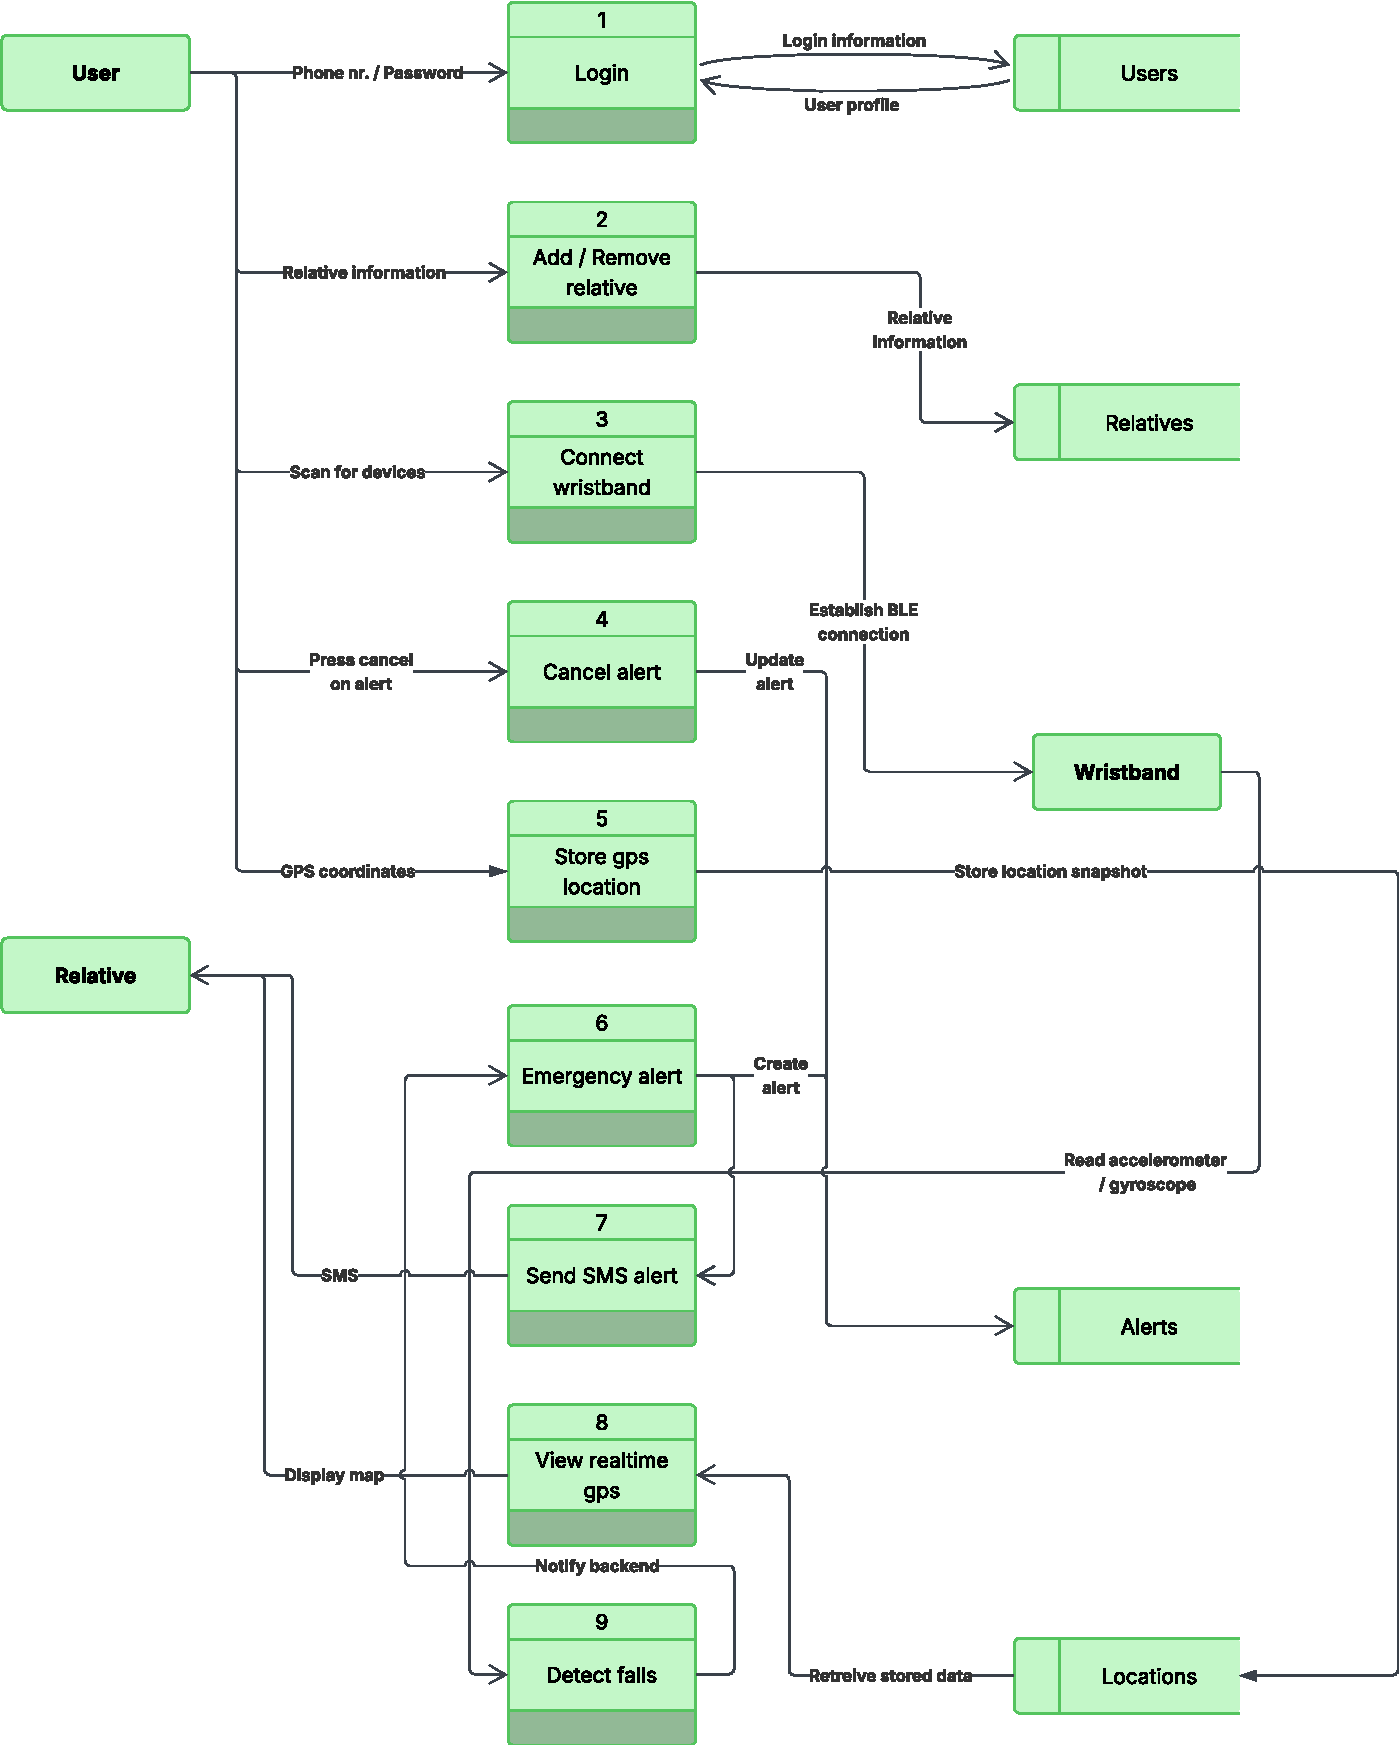
\includegraphics[width=1\linewidth]{Dataflow-Diagram-med-line-jumps.pdf}
    \caption{Data flow diagram over Lapsus}
    \label{fig:placeholder}
\end{figure}

\subsubsection{Sequence diagram}
The sequence diagram below describes the sequence when a fall is detected. The fall is detected by the wristband, which then notifies the mobile app. The mobile app creates the alert, and a new entry is created in the database in the backend. After this, the backend alerts the relative, where they can then respond to the alert. The ‘optional’ shows how a fall can be canceled by the user, in which case the mobile app cancels the alert, and the backend updates the corresponding database entry. After this, the backend notifies the relative, who can then contact the user regarding the canceled alert.  
\begin{figure}[H]
    \centering
    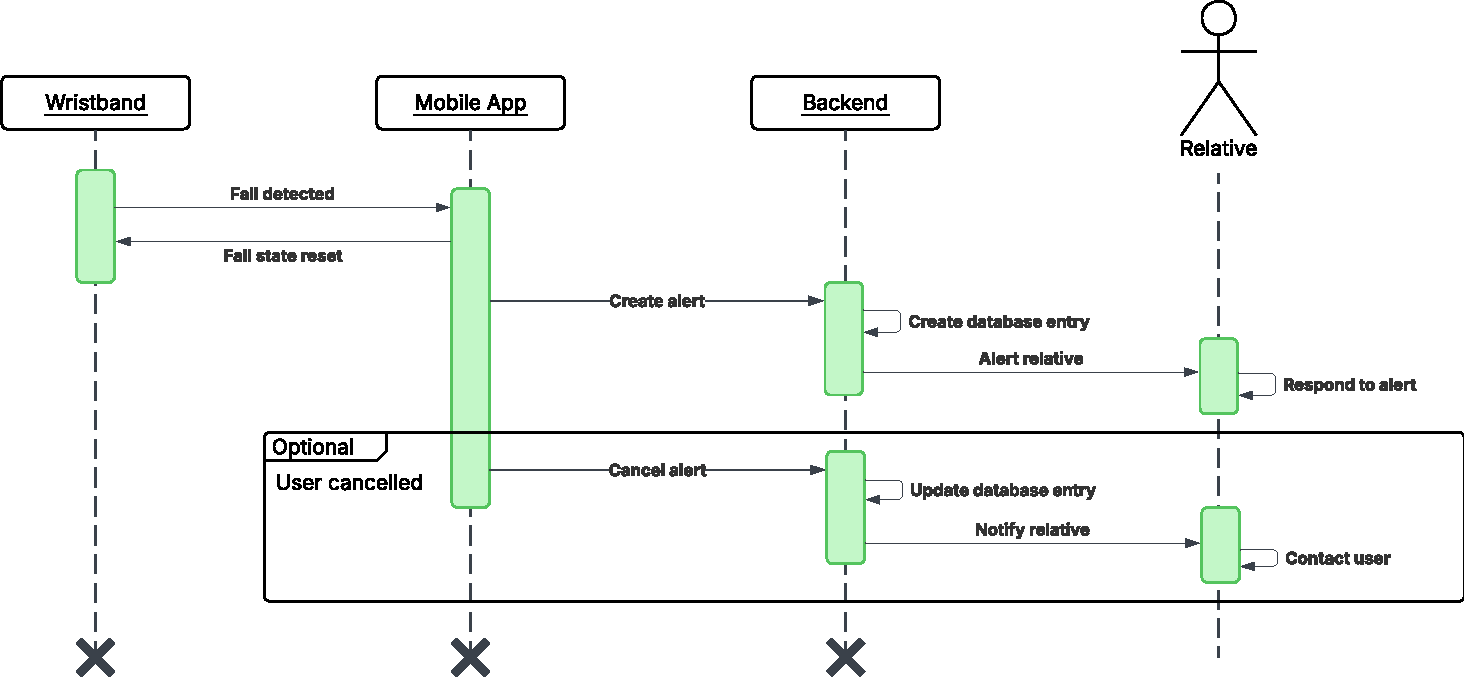
\includegraphics[width=1\linewidth]{Sequence-Diagram-Sequence-Diagram.pdf}
    \caption{Enter Caption}
    \label{fig:placeholder}
\end{figure}

\subsubsection{Deployment diagram}
In the following deployment diagram, 
\begin{figure} [H]
    \centering
    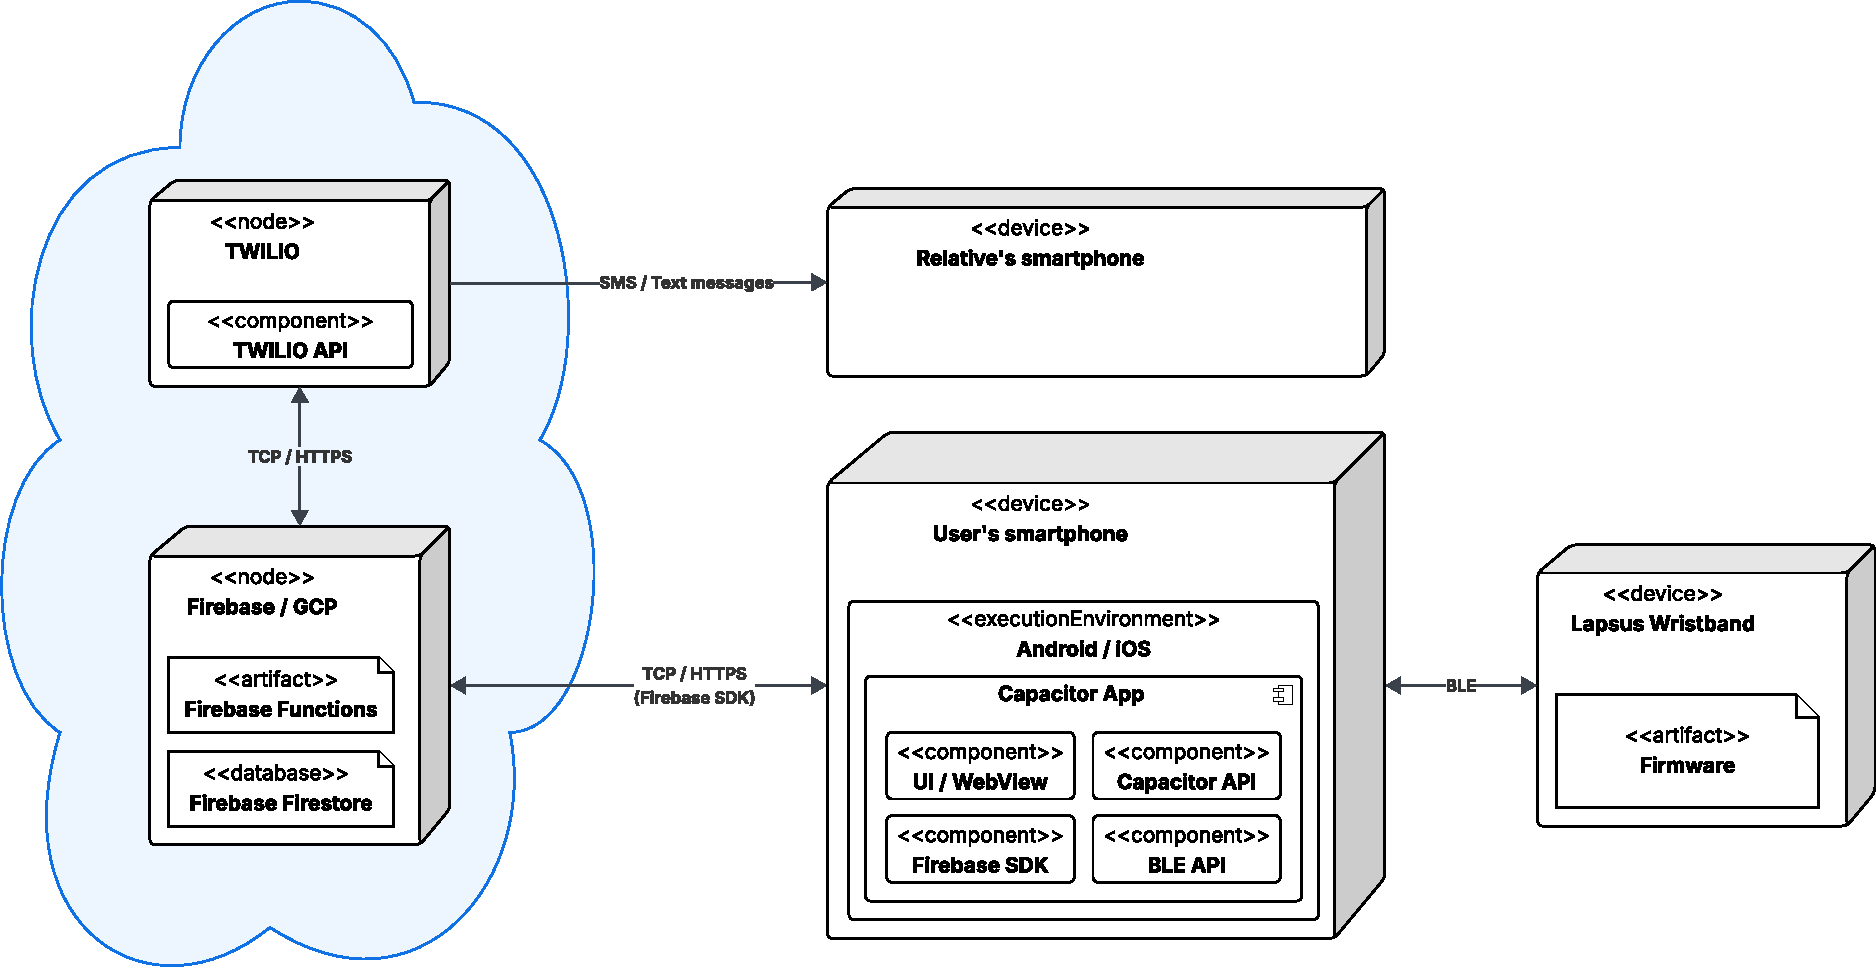
\includegraphics[width=1\linewidth]{Deployment-Diagram-Deployment-Diagram.pdf}
    \caption{Enter Caption}
    \label{fig:placeholder}
\end{figure}